% Para facilitar a manutenção é sempre melhore criar um arquivo por capitulo, para exemplo isso não é necessário

%---------------------------------------------------------------------------------------
\chapter{Descrição da execução do experimento}
	Montou-se o circuito combinacional conforme a \autoref{fig:desenhoCircuito} em uma
	\textit{protoboard}, que possui a \autoref{table:combinacional} como resultado do circuito.

	\begin{figure}[H]
		\centering
		\caption{\label{fig:desenhoCircuito}Desenho do circuito.}
		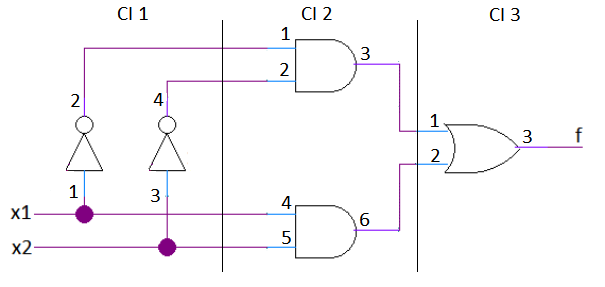
\includegraphics[width=1\textwidth]{img/DesenhoCircuito}
	\end{figure}

	\begin{table}[h]
		\centering
		\caption{Tabela verdade do circuito combinacional.}
		\label{table:combinacional}
		\begin{tabular}{c|c|c}
	%\hline
			\textbf{X1} & \textbf{X2} & \textbf{F}\\
			\hline
			0 & 0 & 1 \\
			0 & 1 & 0 \\
			1 & 0 & 0 \\
			1 & 1 & 1 \\
		\end{tabular}
	\end{table}

	Foram necessários os seguintes equipamentos para o desenvolvimento do experimento:
	\begin{itemize}
		\item Multímetro Digital;
		\item \ac{ci} de portas lógicas \textit{AND} ( \textit{datasheet} 7400 );
		\item \ac{ci} de portas lórigas \textit{OR};
		\item \ac{ci} de porta lógica inversora / \textit{NOT}( \textit{datashee} 7404);
		\item \textit{Protoboard};
		\item Fios para conectar as portas;
		\item Fonte de Alimentação DC 5V;
		\item Alicate.
	\end{itemize}

	Foram realizadas medições das tensões em cada um dos pinos, com multímetro e com osciloscópio,
	do circuito com as entradas x1x2=00, x1x2=01, x1x2=10 e x1x2=11. Observação: Mediu-se as tensões
	usando a faixa de 1000V para ter-se um resultado inteiro.

	\textbf{Obsevação:} Teve-se dificuldade para fotografar as medições, visto que não tinha-se o equipamento necessário
	e não conseguiu-se outra data para e reexecução do experimento.


%Apresentar   o   detalhamento   da  execução  e   resultados   dos   passos   realizados
%durante   o   experimento,   incluindo   tabelas   verdade,   esquemáticos,   e   código
%(quando  houver).
%Especificar  componentes,  sistemas  e  instrumentos  utilizados.
%Usar listas, figuras e quadros, descrevê-los e discuti-los.



%---------------------------------------------------------------------------------------
